\documentclass[a4paper]{report}
\usepackage{graphicx}
\usepackage{array}
\usepackage{natbib}
\usepackage{hyperref}
\usepackage[english]{babel}
\usepackage{lscape}
\usepackage{longtable}

\begin{document}
\begin{titlepage}
\begin{center}
\textsc{\LARGE Contextproject Programming Life}\\
\vspace{5pt}
\textsc{\LARGE Group 2 - GEVATT}\\
\vspace{5pt}
\textsc{\LARGE Final Report}\\
\vspace{5pt}
\textsc{\large TU Delft}

\begin{table}[ht]
\centering
\begin{tabular}{ccc}

\includegraphics[scale=0.2]{ruben.png}   &
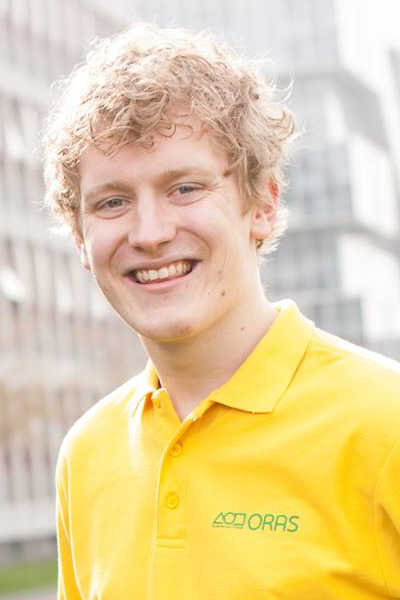
\includegraphics[scale=0.2]{mathijs.png} &

\includegraphics[scale=0.2]{jasper.png}  \\
Ruben Bes	& Mathijs Hoogland	& Jasper Denkers\\
rbes 		& mhhoogland 		& jdenkers\\
4227492 	& 4237676 			& 4212584\\
\end{tabular}
\end{table}

\begin{table}[ht]
\centering
\begin{tabular}{cc}
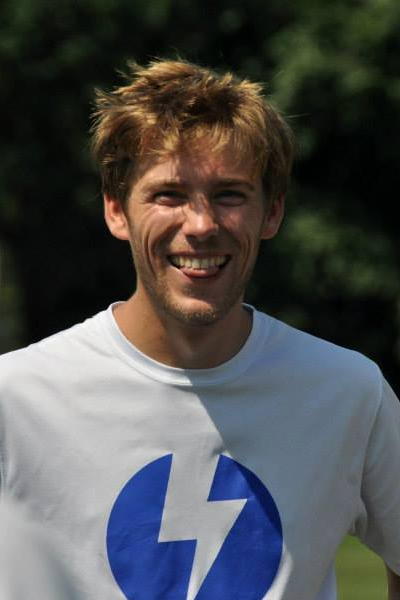
\includegraphics[scale=0.2]{robbert.png} &

\includegraphics[scale=0.2]{willem.png}  \\
Robbert van Staveren	& Willem Jan Glerum\\
rhvanstaveren 			& wglerum\\
1527118					& 4141040\\
\end{tabular}
\end{table}

\vfill
{\large \today}
\end{center}

\end{titlepage}

\begin{landscape}
\setlength\extrarowheight{5pt}
\begin{longtable}{p{6cm}|l|l|l|p{2cm}|p{7cm}}

\textbf{Task} & \textbf{Effort} & \textbf{Assignment} & \textbf{Actual effort} & \textbf{Done} & \textbf{Notes}\\
\hline \hline

Delete patients functionality via Ajax & 1 & Jasper & 2 hours & Yes & None\\
Prevent application from displaying incorrectly on low resolutions & 2 & Jasper & 2 hours & Yes & None\\
Implement JSON protocol between server and client & 2 & Jasper & 0 hours & No & Not started yet\\
Make start a with visualization trio data with mutations unique for the child. Visualization should view the position of SNPs relative to genes & 8 & Jasper and Willem Jan & 20 hours & Yes & Jasper made mutation overview, and Willem Jan made a basic position. This is only basic, needs to be enhanced next week.\\
Upload functionality and apply Robbert's code to process VCF files & 4 & Jasper & 4 hours & Yes & Able to upload and process files, some problems with integrating the VCF reader.\\
Look up visualization library & 3 & Willem Jan & 4 hours & Yes & Looked at multiple libraries and found 3D together with Mathijs\\
Test play in combination with databases & 2 & Willem Jan & 8 hours & No & Spend lot of time, and Ruben as well but doesn't work with mocking the database because of play integration. Other test also depend on the database.\\
Link string and snp database & 2 & Ruben en Robbert & 4 hours & Yes & Quickly done once we found out which elements the databases have in common\\
Retrieve proteins and relevant connections from string data for visualization & 3 & Ruben en Robbert & 4 hours & Yes & No problems once the connection between SNPs and genes/proteins was found\\
Retrieve genes affected by mutations from snp database for visualization & 3 & Ruben en Robbert & 5 hours & Yes & None\\
Look for a way to save retrieved data & 2 & Ruben en Robbert & 1 hour & No & Haven't come to it yet, need to know what data will be retrieved in order to save it. We have found out it is possible to save as a cookie with Play\\
Start visualization of relation between proteins & 6 & Mathijs & 3 hours & No & Have started, but not yet done \\
Start visualization of different chromosomes & 6 & Mathijs & 6 hours & Yes & Made chromosome overview \\
\end{longtable}
\end{landscape}
\end{document}